%%% AgriHome — System Requirements Specification (updated release, Summer 2026)
%%% Structure aligned with CSE 4316 / UTA senior design SRS template

\documentclass[11pt,letterpaper]{article}
\usepackage[margin=1.0in]{geometry}
\usepackage[T1]{fontenc}
\usepackage[utf8]{inputenc}
\usepackage{array}
\usepackage{booktabs}
\usepackage{longtable}
\usepackage{xcolor}
\usepackage{graphicx}
\usepackage{float}
\usepackage[hidelinks]{hyperref}
\usepackage{fancyhdr}
\usepackage{lastpage}
\usepackage{tikz}
\usetikzlibrary{arrows.meta,positioning}

\graphicspath{{images/}}

\definecolor{accentcolor}{rgb}{0.0,0.0,0.5}
\definecolor{leafgreen}{RGB}{61,159,108}

\newcommand{\teamname}{AgriHome}
\newcommand{\coursename}{CSE 4316: Senior Design I}
\newcommand{\semester}{Summer 2026}
\newcommand{\docname}{System Requirements Specification}
\newcommand{\department}{Department of Computer Science \& Engineering}
\newcommand{\university}{The University of Texas at Arlington}
\newcommand{\authors}{%
  GOVINDA AWASTHI\\
  LAXMAN BHUSHAL\\
  THUC DANG\\
  SAGAR KHADKA\\
  MUHAMMAD SAAD MEMON\\
  ALEX TABLIZO\\
  NATHAN NGUYEN TRAN}

\pagestyle{fancy}
\lhead{}
\chead{}
\rhead{}
\lfoot{\footnotesize \teamname\ - \semester}
\cfoot{}
\rfoot{\footnotesize page \thepage\ of \pageref{LastPage}}
\renewcommand{\headrulewidth}{0.0pt}
\renewcommand{\footrulewidth}{0.4pt}

% Compact requirement block helper
\newcommand{\reqblock}[5]{%
\subsubsection{Description} #1
\subsubsection{Source} #2
\subsubsection{Constraints} #3
\subsubsection{Standards} #4
\subsubsection{Priority} #5
}

\begin{document}

{\centering \huge \color{accentcolor} \scshape \textbf{\department \\ \university} \par}
\vspace{0.65in}
{\centering \huge \color{accentcolor} \scshape \textbf{\docname \\ \coursename \\ Spring 2026 (updated \semester)} \par}
\vspace{0.4in}
\begin{center}
	
\includegraphics[width=0.52\textwidth]{agrihome-logo}\\[0.55em]
	{\small\slshape AgriHome project logo: leaf and camera lens motif for vision-based agricultural monitoring.}
\end{center}
\vspace{0.45in}
{\centering \huge \color{accentcolor} \scshape \textbf{\teamname} \par}
\vspace{0.25in}
{\centering \large \scshape \textbf{\authors} \par}
\newpage

\section*{Revision History}
\begin{center}
\begin{tabular}{@{}llll@{}}
\toprule
\textbf{Revision} & \textbf{Date} & \textbf{Author(s)} & \textbf{Description} \\
\midrule
0.1 & 03.2026 & Team & Document creation from charter scope \\
0.2 & 03.2026 & Team & Complete draft \\
0.3 & 03.2026 & Team & Release candidate 1 \\
1.0 & 03.2026 & Team & Official release \\
1.1 & 04.2026 & Team & Customer change requests \\
2.0 & 07.23.2026 & Team & Summer update: edge device requirements 3.10--3.15; security \& future items \\
2.1 & 07.28.2026 & Team & Klipper edge: fswebcam primary capture; klipper\_url / updateKlipperUrl \\
\bottomrule
\end{tabular}
\end{center}
\newpage

\tableofcontents
\newpage
\listoffigures
\listoftables
\newpage

\section{Product Concept}
\subsection{Purpose and Use}
AgriHome is a smart plant monitoring product that helps growers and lab operators observe plant
health continuously, capture tray imagery from edge hardware, and review diagnoses when computer
vision is configured. Users interact primarily through the Vision Console web application. Raspberry
Pi devices running Agri-Home/klipper and \texttt{fswebcam} (via \texttt{agrihome\_agent}) act as
capture endpoints that auto-provision into trays and deliver images through authenticated device APIs.

\subsection{Intended Audience}
\begin{itemize}
  \item Greenhouse operators and facility technicians monitoring multiple trays.
  \item Home gardeners seeking early visual issue detection without constant manual inspection.
  \item Educational agricultural programs and senior-design stakeholders evaluating applied CV systems.
  \item Developers and integrators extending schedules, meshes, or inference backends.
\end{itemize}

\section{Product Description}
\subsection{Features \& Functions}
Core product capabilities through Summer 2026 include:
\begin{itemize}
  \item Authenticated Vision Console (dashboard, trays, plants, mesh, schedule, Devices, settings).
  \item PostgreSQL-backed domain data for trays, plants, captures, reports, events, and edge devices.
  \item Automatic and on-demand image capture via edge devices and capture schedules (including
        destination \texttt{raspberry-pi-edge}).
  \item Operator Take Picture with primary Pi agent + \texttt{fswebcam} path and optional HTTP
        streamer still when \texttt{klipper\_url} is reachable.
  \item Optional species/disease classification via \texttt{cv-backend} / \texttt{CV\_SPECIES\_INFERENCE\_URL},
        including post-ingest disease detection when \texttt{DEVICE\_AUTO\_DISEASE\_ON\_INGEST} is enabled
        (default on).
  \item Historical monitoring display, alerts/events in-console, and plant detail workflows.
  \item Secure edge provisioning (\texttt{POST /api/raspberry-pi/register} +
        \texttt{DEVICE\_PROVISIONING\_SECRET}; model default \texttt{raspberry-pi-klipper}), hashed
        device API keys, heartbeat, and Devices UI (Klipper/streamer URL, poses, schedules).
\end{itemize}

\subsection{External Inputs \& Outputs}
\textbf{Inputs:} user credentials (Firebase), plant/tray metadata, schedule configuration, agent
\texttt{fswebcam} JPEGs (and optional HTTP streamer stills), agent heartbeats, multipart image uploads,
optional CV inference responses.

\textbf{Outputs:} dashboard health status, capture URLs under \texttt{/api/files/...}, plant reports,
monitoring events, device online/offline status, queued edge commands, optional classification labels
and recommendations.

\subsection{Product Interfaces}
\begin{itemize}
  \item Web UI (Next.js App Router PWA) over HTTPS.
  \item REST API routes under \texttt{/api/*} (session cookie for operators; device key header for Pi).
  \item Optional GraphQL endpoint for selected reads/mutations.
  \item Agri-Home/klipper on the Pi (\texttt{fswebcam} / \texttt{save\_image.sh}); optional LAN HTTP
        streamer base stored as \texttt{klipper\_url}.
  \item Optional HTTP inference service (\texttt{CV\_SPECIES\_INFERENCE\_URL}, tray vision URL).
\end{itemize}

\begin{figure}[H]
\centering
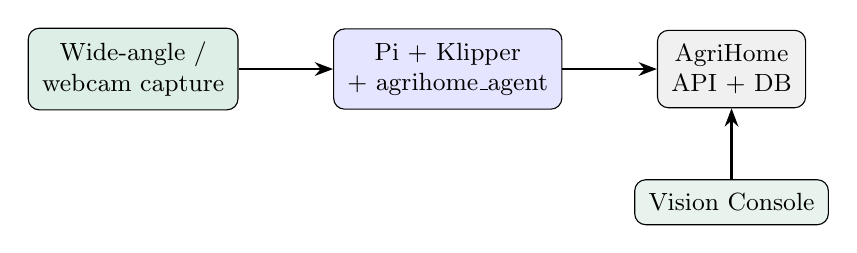
\begin{tikzpicture}[font=\small, box/.style={draw,rounded corners,align=center,inner sep=5pt}, arr/.style={-{Stealth},thick}]
\node[box,fill=leafgreen!18] (cam) {Wide-angle /\\webcam capture};
\node[box,fill=blue!10,right=1.2cm of cam] (edge) {Pi + Klipper\\+ agrihome\_agent};
\node[box,fill=gray!12,right=1.2cm of edge] (ah) {AgriHome\\API + DB};
\node[box,fill=leafgreen!12,below=0.9cm of ah] (ui) {Vision Console};
\draw[arr] (cam) -- (edge);
\draw[arr] (edge) -- (ah);
\draw[arr] (ui) -- (ah);
\end{tikzpicture}
\caption{AgriHome product interfaces: capture hardware, edge agent, API/data plane, and Console.}
\label{fig:srs-arch}
\end{figure}

\section{Customer Requirements}
Customer requirements 3.1--3.9 retain the original SRS intent. Requirements 3.10--3.15 capture the
Summer 2026 Raspberry Pi / Klipper edge integration (auto-provisioning, heartbeat, ingest,
Take Picture via agent/fswebcam, plant upsert/disease detection, and Devices UI with poses/schedules).

\subsection{Plant Health Status Display}
\reqblock
{The system shall provide a user-facing dashboard that displays the current health status of monitored
plants and trays. At minimum, the dashboard shall show a health result such as healthy, warning, or
critical, along with the latest available monitoring result for the user to review.}
{Project Charter, sponsor expectations, and product description.}
{The dashboard must remain simple enough for non-technical users while still showing meaningful
monitoring results. Constrained by frontend development time and prototype scope.}
{Common dashboard usability and readability practices for software systems.}
{Critical}

\subsection{Automatic Image Capture}
\reqblock
{The system shall automatically capture plant images at regular intervals for monitoring purposes.
Operators shall be able to define capture schedules for trays or meshes. Schedules may target the
computer-vision backend path or the \texttt{raspberry-pi-edge} destination so that the schedule runner
enqueues capture work for provisioned Raspberry Pi devices. This requirement supports reducing
constant manual inspection.}
{Product description, project concept, and Summer 2026 edge integration.}
{Image capture reliability depends on camera/webcam hardware, lighting, plant position, agent
\texttt{fswebcam} success, optional streamer reachability, agent heartbeat cadence, processing, and
storage resources.}
{Hardware operating specifications from the selected camera/webcam stack; AgriHome schedule and
edge command contracts.}
{Critical}

\subsection{Environmental Data Collection}
\reqblock
{The system shall collect environmental sensor data associated with plant monitoring when sensors are
available. Data may include temperature, humidity, soil moisture, or related conditions used for
monitoring and analysis.}
{Product description and hardware interface requirements.}
{Depends on successful sensor integration, calibration, and communication with the processing unit.
Sensor quality and hardware cost may affect completeness and accuracy. Not required for the Pi
webcam capture path to function.}
{Manufacturer specifications and standard embedded sensor interfacing practices.}
{High}

\subsection{Alert Display}
\reqblock
{The system shall display alerts or notifications when abnormal plant conditions are detected. Alerts
shall be visible through the dashboard/monitoring views and indicate that a plant or tray may require
attention.}
{Product description, customer need, and sponsor expectations.}
{Alert usefulness depends on detection quality and avoiding excessive false positives that cause alarm
fatigue.}
{Common notification UX practices for monitoring dashboards.}
{Critical}

\subsection{Historical Data Display}
\reqblock
{The system shall display historical monitoring data so users can review trends over time, including
prior captures, reports, and monitoring events associated with trays and plants.}
{Product description and decision-support goals.}
{Retention is limited by storage capacity and prototype scope; visualization complexity is bounded by
UI sprint capacity.}
{Standard time-series / history presentation practices for monitoring tools.}
{High}

\subsection{User Settings Input}
\reqblock
{The system shall allow authenticated users to configure settings relevant to monitoring, such as
schedules, preferences (e.g., ML feedback participation), and account session controls.}
{Product description and usability goals.}
{Settings surface area is constrained to features implemented in the Vision Console; advanced
facility-wide RBAC remains future work.}
{Standard form validation and authenticated configuration practices.}
{High}

\subsection{Dashboard Interface}
\reqblock
{The system shall provide a cohesive dashboard interface summarizing tray health, recent imagery when
available, and navigation to trays, plants, mesh, schedules, and devices.}
{Project Charter and customer usability expectations.}
{Must remain responsive on mobile and desktop within the AppShell layout constraints.}
{Responsive web / PWA usability guidelines.}
{Critical}

\subsection{No Physical Plant Actuation}
\reqblock
{The monitoring product shall not perform physical plant interventions such as automated watering,
fertilizer dosing, or pesticide application as part of the core prototype scope. Pose/hinge/motor
controls on the capture rig, when present, are for camera positioning only and remain stubbed or
operator-supervised.}
{Safety review and project scope boundaries.}
{Hardware motion subsystems must not be presented as autonomous plant-care actuators.}
{Laboratory safety practices; RIA-oriented manipulator caution where motion hardware exists.}
{Critical}

\subsection{Remote Notification Support}
\reqblock
{In a future version, the system should support remote notification delivery such as email, mobile push,
or text message when abnormal plant conditions are detected, allowing alerts when the dashboard is
not open.}
{Future customer convenience needs and product expansion goals.}
{Requires additional backend services, notification platform integration, secure internet
communication, and account support; may not be feasible within current prototype scope.}
{Secure communication practices and standard authentication methods.}
{Future}

\subsection{Edge Device Auto-Provisioning}
\reqblock
{The system shall auto-provision Raspberry Pi edge devices via
\texttt{POST /api/raspberry-pi/register}. Agents present a hardware fingerprint (CPU serial required;
MAC/hostname/model/\texttt{klipperUrl} optional; model defaults to \texttt{raspberry-pi-klipper}) and a provisioning code that must match
\texttt{DEVICE\_PROVISIONING\_SECRET}. Successful provisioning shall create an \texttt{edge\_devices}
record, issue a device API key (plaintext returned once), store only the SHA-256 hash of that key,
and create or link a tray for monitoring. Re-provision of an existing serial shall require an explicit
\texttt{reProvision} flag.}
{Summer 2026 Hardware \& Software Integration (Pi) sprint; ops threat model AGRI-109.}
{Open registration shall be rejected when \texttt{DEVICE\_PROVISIONING\_SECRET} is unset. Duplicate
serial without \texttt{reProvision} shall fail safely (HTTP~409). Owner email assignment must follow
\texttt{DEVICE\_DEFAULT\_OWNER\_EMAIL} or an explicit register payload. Registration must never create
a Firebase/human user account.}
{Least-privilege device onboarding; secret rotation practices (see Edge Device Security notes).}
{Critical}

\subsection{Device Heartbeat and Online Status}
\reqblock
{Provisioned devices shall send periodic heartbeats to \texttt{POST /api/raspberry-pi/heartbeat}
authenticated with the device API key header (\texttt{X-Agrihome-Device-Key}). The system shall update
last-heartbeat timestamps and derive online/offline (or stale) status for display in the Vision Console.
Heartbeat responses shall include pending edge commands for the agent to claim when requested.}
{Edge reliability and operator situational awareness needs (AGRI-103).}
{Status freshness depends on agent cadence and \texttt{DEVICE\_HEARTBEAT\_STALE\_MINUTES}
configuration. Network partitions may delay status transitions. Revoked devices must be rejected.}
{Standard keep-alive / device presence patterns for IoT-style agents.}
{Critical}

\subsection{Secure Multipart Image Ingest}
\reqblock
{The system shall accept multipart image uploads from provisioned devices at
\texttt{POST /api/raspberry-pi/ingest} authenticated with \texttt{X-Agrihome-Device-Key}. Uploads shall
be size-limited (\texttt{DEVICE\_INGEST\_MAX\_BYTES}) and rate-limited per device and per IP
(\texttt{DEVICE\_INGEST\_MAX\_PER\_DEVICE\_PER\_MIN}, \texttt{DEVICE\_INGEST\_MAX\_PER\_IP\_PER\_MIN}).
Successful ingest shall persist image bytes under configured storage, create corresponding capture
records, and may complete a claimed edge command when a \texttt{commandId} is supplied.}
{Edge capture pipeline; security hardening AGRI-109 / AGRI-101.}
{Device keys are verified against stored SHA-256 hashes; plaintext keys are not re-readable from the
database. Revoked devices must be rejected. Storage capacity and max byte limits constrain burst
uploads. Excess traffic shall return HTTP~429 with retry guidance.}
{TLS in transit where terminated; authenticated upload best practices; rate limiting.}
{Critical}

\subsection{Operator Take Picture Command}
\reqblock
{Authenticated operators shall be able to trigger Take Picture for a tray-linked edge device from the
Vision Console (device action \texttt{capture} on \texttt{POST /api/devices/\{id\}}). The primary path shall
queue a \texttt{capture\_now} command for the Pi agent, which captures with \texttt{fswebcam} via
Agri-Home/klipper \texttt{camera-macros/save\_image.sh} and uploads via ingest. When an optional HTTP
streamer base is stored as \texttt{klipper\_url} and reachable from the AgriHome host, the system may
attempt a server-side still first (\texttt{AGRIHOME\_SNAPSHOT\_PATH} / timeout configuration) before
queuing the agent.}
{Operator workflow; Raspberry Pi + Klipper integration guide (\texttt{docs/ops/RASPBERRY\_PI\_KLIPPER.md}).}
{Agent capture latency is bounded by heartbeat interval. Optional server-side stills require LAN
reachability to the streamer URL. Deprecated aliases \texttt{moonrakerUrl} / \texttt{updateMoonrakerUrl}
remain accepted.}
{Agri-Home/klipper camera-macros; AgriHome device action API contract (\texttt{updateKlipperUrl}).}
{Critical}

\subsection{Automatic Plant Upsert and Disease Detection after Pi Capture}
\reqblock
{After a successful Pi capture ingest (or server-side Take Picture persistence), the system shall
automatically upsert/attach a plant on the linked tray when plant identity can be determined or created
per product rules (pose/slot-aware attach). When \texttt{DEVICE\_AUTO\_DISEASE\_ON\_INGEST} is enabled
(default true), the system shall run leaf species/disease classification asynchronously and persist
prediction/report outputs. Optional tray vision may also run when
\texttt{DEVICE\_AUTO\_VISION\_ON\_INGEST} is enabled and inference URLs are configured.}
{Summer 2026 CV + edge integration (AGRI-107).}
{CV quality depends on model training data and lighting. Auto-disease or auto-vision may be disabled
by configuration. Auto-upsert behavior must not corrupt unrelated trays or owners.}
{Documented inference JSON contracts for \texttt{cv-backend}; data integrity for plant/tray foreign keys.}
{High}

\subsection{Edge Device Management UI, Klipper URL, Poses \& Schedules}
\reqblock
{The Vision Console shall provide edge device management surfaces including a Devices navigation
entry listing provisioned devices (serial, status, last heartbeat, linked tray) and a tray-level
Raspberry Pi panel supporting Take Picture, device linking, Klipper/streamer URL edit/save
(\texttt{updateKlipperUrl}; deprecated alias \texttt{updateMoonrakerUrl}), and clear empty/offline states.
Operators shall be able to configure capture pose sequences for trays and create schedules with
destination \texttt{raspberry-pi-edge} so the schedule runner enqueues multi-angle \texttt{capture\_now} work.
Device agents shall obtain active poses and capture plans via authenticated
\texttt{/api/raspberry-pi/poses} and \texttt{/api/raspberry-pi/capture-plan} endpoints.}
{Operator usability; AGRI-104 / AGRI-105 / AGRI-106.}
{UI must respect authentication and ownership. Klipper URL updates must validate http/https
URLs. Offline devices should present clear empty states rather than silent failures. Pose generation
depends on tray plant layout data.}
{Responsive AppShell navigation patterns already used by the Console.}
{High}

\section{Packaging Requirements}
The finished product includes a camera/webcam fixture (optionally mounted with lighting), access to
the Vision Console from any modern web browser, and optional AI image processing via a configured
inference host. Hardware packaging may require user adjustment of mounting points for shelf
attachment. Software packaging is a deployable Next.js application with environment configuration,
database migrations, and an edge agent reference package.

\subsection{Hardware Packaging}
\reqblock
{Hardware for the camera system will be partially assembled; mounting the fixture may require
adjustment by the user. The package should include custom mounting hardware appropriate to the
shelf/tray design. Raspberry Pi + Agri-Home/klipper + \texttt{fswebcam} stacks are expected as bench capture units.}
{Project Charter.}
{Packaging size and assembly complexity restrict how many parts can be pre-assembled.}
{None beyond maker-space fabrication norms.}
{Medium}

\subsection{Software Packaging}
\reqblock
{Access to the main control interface shall be provided as a web application (Vision Console) with
documented environment variables, database migrations, and optional container/CI build artifacts.
Edge devices shall use the \texttt{agrihome\_agent} reference package for register/run workflows.}
{Project Charter and implementation guide.}
{Deployment depends on PostgreSQL availability, Firebase configuration, and network access between
Console host and Pi agent; optional when using server-side streamer stills.}
{Standard web application packaging and 12-factor style configuration.}
{High}

\section{Performance Requirements}
\subsection{Reliability}
\reqblock
{Core monitoring reads/writes shall remain available when optional CV services are down. Edge ingest
and heartbeat shall fail closed on invalid credentials. Stale devices shall be markable offline after the
configured heartbeat window.}
{Operational robustness goals.}
{Single-host prototype deployments remain a single point of failure unless operators add redundancy.}
{Graceful degradation practices for optional dependencies.}
{High}

\subsection{Speed}
\reqblock
{Dashboard and tray pages shall load interactive shells within interactive web expectations on lab
networks. Take Picture should complete via agent \texttt{fswebcam} ingest within a small number of
heartbeat intervals under normal bench conditions; when an optional streamer URL is reachable,
server-side stills may return an image URL immediately.}
{Usability goals.}
{WAN latency, WARP/VPN LAN overrides, and Pi CPU load can delay snapshots and uploads.}
{Reasonable interactive web performance; no hard real-time guarantees.}
{High}

\section{Safety Requirements}
\subsection{Laboratory Equipment Lockout/Tagout (LOTO) Procedures}
\reqblock
{Team members shall follow applicable laboratory LOTO practices when servicing powered fixtures,
lighting, or motion hardware associated with the capture rig.}
{University laboratory safety policy.}
{Student access hours and training availability may limit when hardware can be serviced.}
{UTA lab safety / LOTO guidance.}
{Critical}

\subsection{National Electric Code (NEC) Wiring Compliance}
\reqblock
{Electrical assembly for lighting and device power shall follow safe wiring practices consistent with
applicable NEC guidance for the installation context (prototype bench, not a permanent building
modification unless approved).}
{Facilities and safety review.}
{Prototype wiring must remain inspectable and not overload lab circuits.}
{NEC-informed safe wiring practices for low-voltage/prototype setups.}
{High}

\subsection{RIA Robotic Manipulator Safety Standards}
\reqblock
{If hinge/motor positioning hardware is energized, operators shall treat it as motion equipment:
maintain clearance, avoid unsupervised autonomous sweeps near people, and keep plant-care actuation
out of scope (see requirement 3.8).}
{Safety scope boundary.}
{Pose control may be stubbed; physical motion capability varies by bench build.}
{RIA-oriented manipulator safety caution for educational prototypes.}
{High}

\section{Security Requirements}
This section defines security and privacy requirements for AgriHome. The system captures plant
images and processes data through backend services. Controls protect user sessions, device credentials,
and stored imagery.

\subsection{User Authentication}
\reqblock
{The system shall require user authentication to access the dashboard and protected system data. Users
must sign in (Firebase email/password or Google) before accessing plant monitoring information;
server routes shall verify session cookies.}
{System security and user access control requirements.}
{Authentication must remain usable for operators while maintaining adequate security. Password reset
and full RBAC remain partially future.}
{Standard authentication practices; Firebase Auth guidance.}
{Critical}

\subsection{Data Encryption}
\reqblock
{Data transmitted between browsers, AgriHome servers, and (where feasible) edge agents shall use TLS
when terminated in front of the application. Sensitive secrets must not be committed to source control.}
{Data protection and privacy requirements.}
{Local bench HTTP may be used on trusted LANs during development; production should prefer TLS.}
{TLS for secure data transmission.}
{Critical}

\subsection{Secure Data Storage}
\reqblock
{Stored data, including plant images and system logs/events, shall be protected against unauthorized
access. Access to stored data must be restricted to authorized users. Device API keys shall be stored
only as SHA-256 hashes in \texttt{edge\_devices.api\_key\_hash}; plaintext keys are returned only once at
register or rotate-key and must not be recoverable from the database. Edge device onboarding shall
require a rotatable \texttt{DEVICE\_PROVISIONING\_SECRET} (open registration disabled when unset).}
{Data privacy, system security, and AGRI-109 Edge Device Security notes.}
{Local filesystem storage security depends on host permissions. Database backups must be handled as
sensitive. Operators should rotate the provisioning secret when personnel leave or a bench is
decommissioned.}
{Secure storage best practices; hashed credential storage.}
{High}

\subsection{Access Control}
\reqblock
{The system shall enforce user-based ownership controls so operators access their trays, plants,
schedules, and devices via Firebase session cookies. Device endpoints
(\texttt{/api/raspberry-pi/*}) shall authenticate with device API keys
(\texttt{X-Agrihome-Device-Key}) distinct from Firebase user identities. Registration must never create
a human account. Operators may revoke or rotate device keys through authenticated device actions.}
{System design and security requirements; AGRI-109.}
{Fine-grained RBAC roles (admin/reviewer/operator) are not fully implemented in the prototype.}
{Access control and authorization best practices.}
{High}

\subsection{System Integrity and Protection}
\reqblock
{The system shall protect integrity of ingest and command flows via hashed device-key authentication,
revoke/rotate key actions, ingest rate limits, maximum upload size, and rejection of invalid
provisioning attempts (including replay of registration without intentional re-provision). Unauthenticated
HTTP streamers and Klipper APIs should not be exposed to the public Internet without authentication.}
{Edge threat model: rogue provisioning, stolen keys, spam uploads (AGRI-109).}
{Rate limits and max bytes are configuration-dependent; operators must rotate secrets when benches
are decommissioned.}
{Defense-in-depth for IoT-style device APIs.}
{High}

\section{Maintenance \& Support Requirements}
\subsection{System Maintenance Documentation}
\reqblock
{The team shall maintain documentation describing deployment, migrations, edge provisioning, and
known networking caveats (e.g., optional streamer URL discovery, WARP LAN overrides, fswebcam device paths).}
{Course deliverable and operational needs.}
{Docs must track Summer 2026 behavior changes; stale docs are a risk.}
{Internal engineering documentation standards.}
{High}

\subsection{Hardware Maintenance and Replacement}
\reqblock
{Webcam/Pi hardware shall be replaceable by re-provisioning or rotating device credentials. Fixtures
should allow camera swap without redesigning the entire rack.}
{Prototype maintainability.}
{Lead time for replacement parts may delay demos.}
{Standard hardware spare strategy.}
{Medium}

\subsection{Software Updates and Bug Fixes}
\reqblock
{Software shall be updatable via normal git-based development, migrations, and redeploy of the Next.js
application and agent package. Critical security fixes for provisioning/ingest shall be prioritized.}
{Maintenance policy.}
{Course bandwidth limits how many non-critical fixes land each sprint.}
{Semantic versioning for documents; conventional deploy practices.}
{High}

\subsection{System Monitoring and Error Logging}
\reqblock
{The system shall expose health checks (e.g., \texttt{/api/health}) reporting database connectivity and
whether inference URLs are configured. Edge online status shall be visible in the Devices UI.
Application errors should be observable in server logs during operation.}
{Operability requirements.}
{Centralized log aggregation is optional for the prototype.}
{Health-check patterns for web services.}
{High}

\subsection{Technical Support Availability}
\reqblock
{During the senior-design project window, team members provide support to stakeholders for demos
and lab use. Post-course support is not guaranteed unless separately arranged.}
{Course staffing reality.}
{Availability follows academic calendars and sprint commitments.}
{None.}
{Medium}

\section{Other Requirements}
\subsection{System Setup and Configuration}
\reqblock
{Operators shall be able to configure environment variables for database, Firebase, storage roots,
\texttt{DEVICE\_PROVISIONING\_SECRET}, default owner email, heartbeat stale window, ingest size/rate
limits, snapshot path/timeout, \texttt{DEVICE\_AUTO\_DISEASE\_ON\_INGEST},
\texttt{DEVICE\_AUTO\_VISION\_ON\_INGEST}, and optional CV URLs before running the application and
agent.}
{Implementation guide and ops docs.}
{Misconfiguration can disable registration or CV/disease paths.}
{12-factor configuration practices.}
{Critical}

\subsection{System Modularity}
\reqblock
{Presentation, application/API, processing (CV), data, and edge agent concerns shall remain separable
so that CV or Pi hardware can be absent without blocking core Console CRUD monitoring.}
{Architectural Design Specification.}
{Some features degrade when optional services are unset.}
{Layered architecture modularity.}
{High}

\subsection{System Extensibility}
\reqblock
{The system shall allow extending schedules, pose sequences, meshes, and inference providers without
rewriting the entire Console.}
{Product roadmap.}
{Extensibility is bounded by schema migrations and API stability.}
{Interface-oriented extension practices.}
{High}

\subsection{Platform Compatibility}
\reqblock
{The Vision Console shall run in modern desktop and mobile browsers. Edge agents target Raspberry Pi
OS-class Linux with Python~3 and network access to AgriHome.}
{Customer accessibility goals.}
{Older browsers and highly locked-down networks may limit PWA install or snapshot reachability.}
{Baseline evergreen browser support; Linux edge runtime.}
{High}

\subsection{Programming Language and Environment}
\reqblock
{Primary application code shall use TypeScript/Next.js with PostgreSQL. CV backend and edge agent
shall use Python as implemented. Build/test should run in the team's documented Node and Python
environments.}
{Team skill set and repository standards.}
{Language/runtime upgrades must not be taken lightly mid-semester.}
{Language and framework documentation for Next.js, PostgreSQL, and Python.}
{High}

\section{Future Items}
This section summarizes features considered but not fully delivered, or only partially implemented, in
the current prototype.

\subsection{Mobile Application Support}
\reqblock
{A dedicated native mobile application could allow monitoring, notifications, and settings without a
browser. The current PWA covers many mobile needs but is not a store-distributed native app.}
{User experience enhancement goals.}
{Requires additional development time and cross-platform packaging.}
{iOS/Android application guidelines.}
{Future}

\subsection{Advanced AI-Based Plant Disease Detection}
\reqblock
{Advanced AI-based plant disease detection is \textbf{partially implemented}: the team trains and serves a
PlantVillage-style multi-class classifier in \texttt{cv-backend} and can invoke it from AgriHome when
\texttt{CV\_SPECIES\_INFERENCE\_URL} is configured, including optional post-Pi-capture detection. Remaining
future work includes broader crop coverage, stronger real-world robustness, richer explainability
(e.g., heatmaps), and production MLOps hardening.}
{Project design discussion; Summer 2026 CV status.}
{Requires datasets, training compute, and careful evaluation under greenhouse lighting.}
{AI/ML best practices and data handling guidelines.}
{Partial / Future}

\subsection{Cloud-Based Data Analytics and Sharing}
\reqblock
{Future versions may add deeper cloud analytics, cross-organization sharing, and multi-site rollups
beyond the current single-tenant-style ownership model.}
{System scalability considerations.}
{Requires additional cloud infrastructure, security review, and ongoing maintenance.}
{Cloud computing and data security standards.}
{Future}

\subsection{Offline Device Alerts (AGRI-110)}
\reqblock
{The system should alert operators when a previously online edge device becomes stale/offline beyond
the heartbeat window (in-console first; optionally email/push later). This item is tracked as
AGRI-110 and is not fully implemented in Revision~2.1.}
{Edge operability gap identified during Pi integration.}
{Requires notification policy, deduplication, and ownership-aware delivery.}
{Monitoring alert practices; reuse future remote notification channels where available.}
{Future}

\newpage
\begin{thebibliography}{9}
\bibitem{charter}
AgriHome, \textit{Project Charter}, CSE~4316 / updated Summer~2026.

\bibitem{ads}
AgriHome, \textit{Architectural Design Specification}, CSE~4316, Spring~2026.

\bibitem{edge-sec}
AgriHome, \textit{Edge Device Security (AGRI-109)}, project operations documentation, 2026.

\bibitem{klipper-ops}
AgriHome, \textit{Raspberry Pi + Klipper} operations guide (\texttt{docs/ops/RASPBERRY\_PI\_KLIPPER.md}), 2026.
\bibitem{moonraker-ops}
AgriHome, \textit{Raspberry Pi + Moonraker} operations guide (superseded stub; see Klipper guide), 2026.

\bibitem{rubin}
K.~S. Rubin, \textit{Essential Scrum}, Addison-Wesley, 2012.

\bibitem{firebase}
Google, ``Firebase Authentication,'' \url{https://firebase.google.com/docs/auth}.

\bibitem{nextjs}
Vercel, Inc., ``Next.js Documentation,'' \url{https://nextjs.org/docs}.
\end{thebibliography}

\end{document}
